\documentclass[]{beamer}
%
% Choose how your presentation looks.
%
% For more themes, color themes and font themes, see:
% http://deic.uab.es/~iblanes/beamer_gallery/index_by_theme.html
%
\mode<presentation>
{
  \definecolor{StanfordCardinal}{RGB}{140, 21, 21} % Stanford Cardinal (primary)
  \usetheme{Madrid}      % or try Darmstadt, Madrid, Warsaw, ...
  \usecolortheme[named=StanfordCardinal]{structure} % or try albatross, beaver, crane, ...
  \usefonttheme{default}  % or try serif, structurebold, ...
  \setbeamertemplate{navigation symbols}{}
  \setbeamertemplate{caption}[numbered]
  %\useinnertheme{circles}
  %\useoutertheme{miniframes} % Alternatively: miniframes, infolines, split
} 
\usepackage{xcolor}
\usepackage[english]{babel}
\usepackage[utf8x]{inputenc}

\title[GSE Math Camp: Day 1]{GSE Math Camp Day 1: \\ Software and Pre-Calculus Review}
\author{Klint Kanopka}
\institute{kkanopka@stanford.edu}
\date{Tuesday, September 3, 2019}

\begin{document}

    \begin{frame}
      \titlepage
    \end{frame}

    \begin{frame}{About Me}
        \begin{center}
        
\includegraphics[scale=0.4]{img/physicists.png}
        \end{center}
    \end{frame}

    \begin{frame}{Personal Information}
        \begin{itemize}
            \item From Philadelphia
            \item Taught physics in the Philadelphia School District for 8 years
            \item $3^{\text{rd}}$ year PhD Student (DAPS)
            \item Also doing MSCS (AI track)
            \item Interested in measurement, assessment, and the intersection of AI and psychometrics
            \item I'm willing to answer almost any question you have (personal or otherwise)
        \end{itemize}
    \end{frame}

    \begin{frame}{Math Camp Materials}
        All materials for the first week are hosted at:
        \url{http://github.com/klintkanopka/gsemathcamp}
    \end{frame}
    
    \begin{frame}{Outline}
      \tableofcontents
    \end{frame}
    
\section{Software Packages of Interest}

    \subsection{Document Processing}

    \begin{frame}{Document Processing}
        \begin{itemize}
            \item<2-> Microsoft Word (the standard)
            \item<3-> \LaTeX (old faithful for scientific papers - and these slides)
            \item<4-> Markdown (newer, least used, but gaining steam)
        \end{itemize}
    \end{frame}

    \subsection{Citation Managers}

    \begin{frame}{Citation Managers}
        These organize your academic papers and help you generate reference lists for papers you're working on.
        \begin{itemize}
            \item<2-> Mendeley
            \item<3-> Zotero
            \item<4-> Endnote
            \item<5-> Stanford library and UToronto library both have good websites describing the different options
        \end{itemize}
    \end{frame}

    \subsection{Quantitative Software}

    \begin{frame}{Quantitative Software}
        \begin{itemize}
            \item<2-> Microsoft Excel
            \item<3-> SPSS (Statistical Package for Social Science) 
            \item<4-> SAS (Statistical Analysis Software)
            \item<5-> Stata
            \item<6-> R
            \item<7-> Python
        \end{itemize}
    \end{frame}

    \subsection{VPN}

    \begin{frame}{VPN}
        Set up Cisco VPN!
        \begin{itemize}
            \item<2-> Allows access to journals, data, library materials, networks from off-campus
            \item<3-> Absolutely necessary if you live off campus or travel
            \item<4-> For instructions: uit.stanford.edu/service/vpn
            \item<5-> If you travel overseas often (and plan on working during that time), also consider a physical 2-factor authentication token (available at ID card office for free)
        \end{itemize}
   \end{frame}

\section{Review of Algebra and Notation}

    \subsection{Order of Operations}

    \begin{frame}{Basic Algebraic Symbols}
        \begin{itemize}
            \item<2-> Addition ($+$)
            \item<2-> Subtraction ($-$)            
            \item<2-> Multiplication ($\times, *$)
            \item<2-> Division ($\div, /$)
            \item<3-> Sum ($\sum$)
            \item<3-> Product ($\prod$)
        \end{itemize}
    \end{frame}

    \begin{frame}{Sums}
        $$ \sum_{n=1}^3 n = 1 + 2 + 3 = 6 $$
        \onslide<2->{$$ N = \{1,2,3\} $$}
        \onslide<3->{$$ \sum_{n\in N} n = 1 + 2 + 3 = 6 $$}
        \onslide<4->{$$ \sum_{i=1}^3 n_i = 1+2+3=6 $$}
        \onslide<5->{Often you'll see generalized sums:
        $$ \sum_{i=1}^N$$}
    \end{frame}

    \begin{frame}{Products}
        $$ \prod_{n=1}^3 n = 1 \times 2 \times 3 = 6 $$
        \onslide<2->{$$ N = \{1,2,3\} $$}
        \onslide<3->{$$ \prod_{n\in N} n = 1 \times 2 \times 3 = 6 $$}
        \onslide<4->{$$ \prod_{i=1}^3 n_i = 1 \times 2 \times 3=6 $$}
        \onslide<5->{Often you'll see generalized products:
        $$ \prod_{i=1}^N$$}
    \end{frame}

    \begin{frame}{Exercises}
        Try these and then check with a partner:
        \begin{enumerate}
            \item Evaluate: $\sum\limits_{x=1}^5 x$ 
            \item Solve for $x$: $50 = 5(x+2) + 5$            
            \item Evaluate: $\prod\limits_{x=1}^3 (x-1)$
        \end{enumerate}
    \end{frame}

\subsection{Working with Units}

    \begin{frame}{Working with Units}
        You're only allowed to add, subtract, or compare quantities of the same unit
        \begin{itemize}
            \item<2-> 1 English Bulldog + 1 Dachshund = ??
            \item<3-> 1 Dog + 1 Dog = 2 Dogs!            
        \end{itemize}
    \end{frame}

    \begin{frame}{Working with Units}
        Units multiply and divide! 
        \begin{itemize}
            \item<2-> Driving 60 miles per hour for 2 hours takes you 120 miles $$60 \frac{miles}{hour} \times 2 hours = 120 miles $$
            \item<3-> A rectangular neighborhood that is 2km by 3km has an area of 6 square km $$2 km \times 3km = 6km^2$$
            \item<4-> Proportions have no units!
        \end{itemize}
    \end{frame}

\subsection{Exponents}

    \begin{frame}{Exponents}
        Rules of exponents:
        \begin{enumerate}
            \item<2-> $a^n = $ \onslide<3->{$\underbrace{a \times a \times \cdots \times a}_n$}
            \item<4-> $a^0 = $ \onslide<5->{$1$} 
            \item<6-> $a^{-1} = $ \onslide<7->{$\frac{1}{a}$}
            \item<8-> $a^{x+y} = $ \onslide<9->{$a^xa^y$}
            \item<10-> $a^{x-y} = $ \onslide<11->{$\frac{a^x}{a^y}$}
            \item<12-> $(a^x)^y = $ \onslide<13->{$a^{xy}$}
            \item<14-> $(ab)^x = $ \onslide<15->{$a^xb^x$}
            \item<16-> $(\frac{a}{b})^x = $ \onslide<17->{$\frac{a^x}{b^x}$}
            \item<18-> $a^{\frac{1}{2}} = $ \onslide<19->{$\sqrt{a}$}
            \item<20-> $\sqrt[x]{a} = $ \onslide<21->{$a^\frac{1}{x}$}
        \end{enumerate}
    \end{frame}

    \begin{frame}{Exercises}
        \begin{enumerate}
            \item Evaluate: $(5\times 4)^2$
            \item Evaluate: $((1+3)^3)^2 \times 2 + 5$
        \end{enumerate}
    \end{frame}

    \subsection{The Coordinate Plane}
    
    \begin{frame}{Coordinate Plane}
        There are four \textbf{quadrants} on a coordinate plane. The horizontal axis is known as the x-axis and the vertical axis is known as the y-axis. \\
            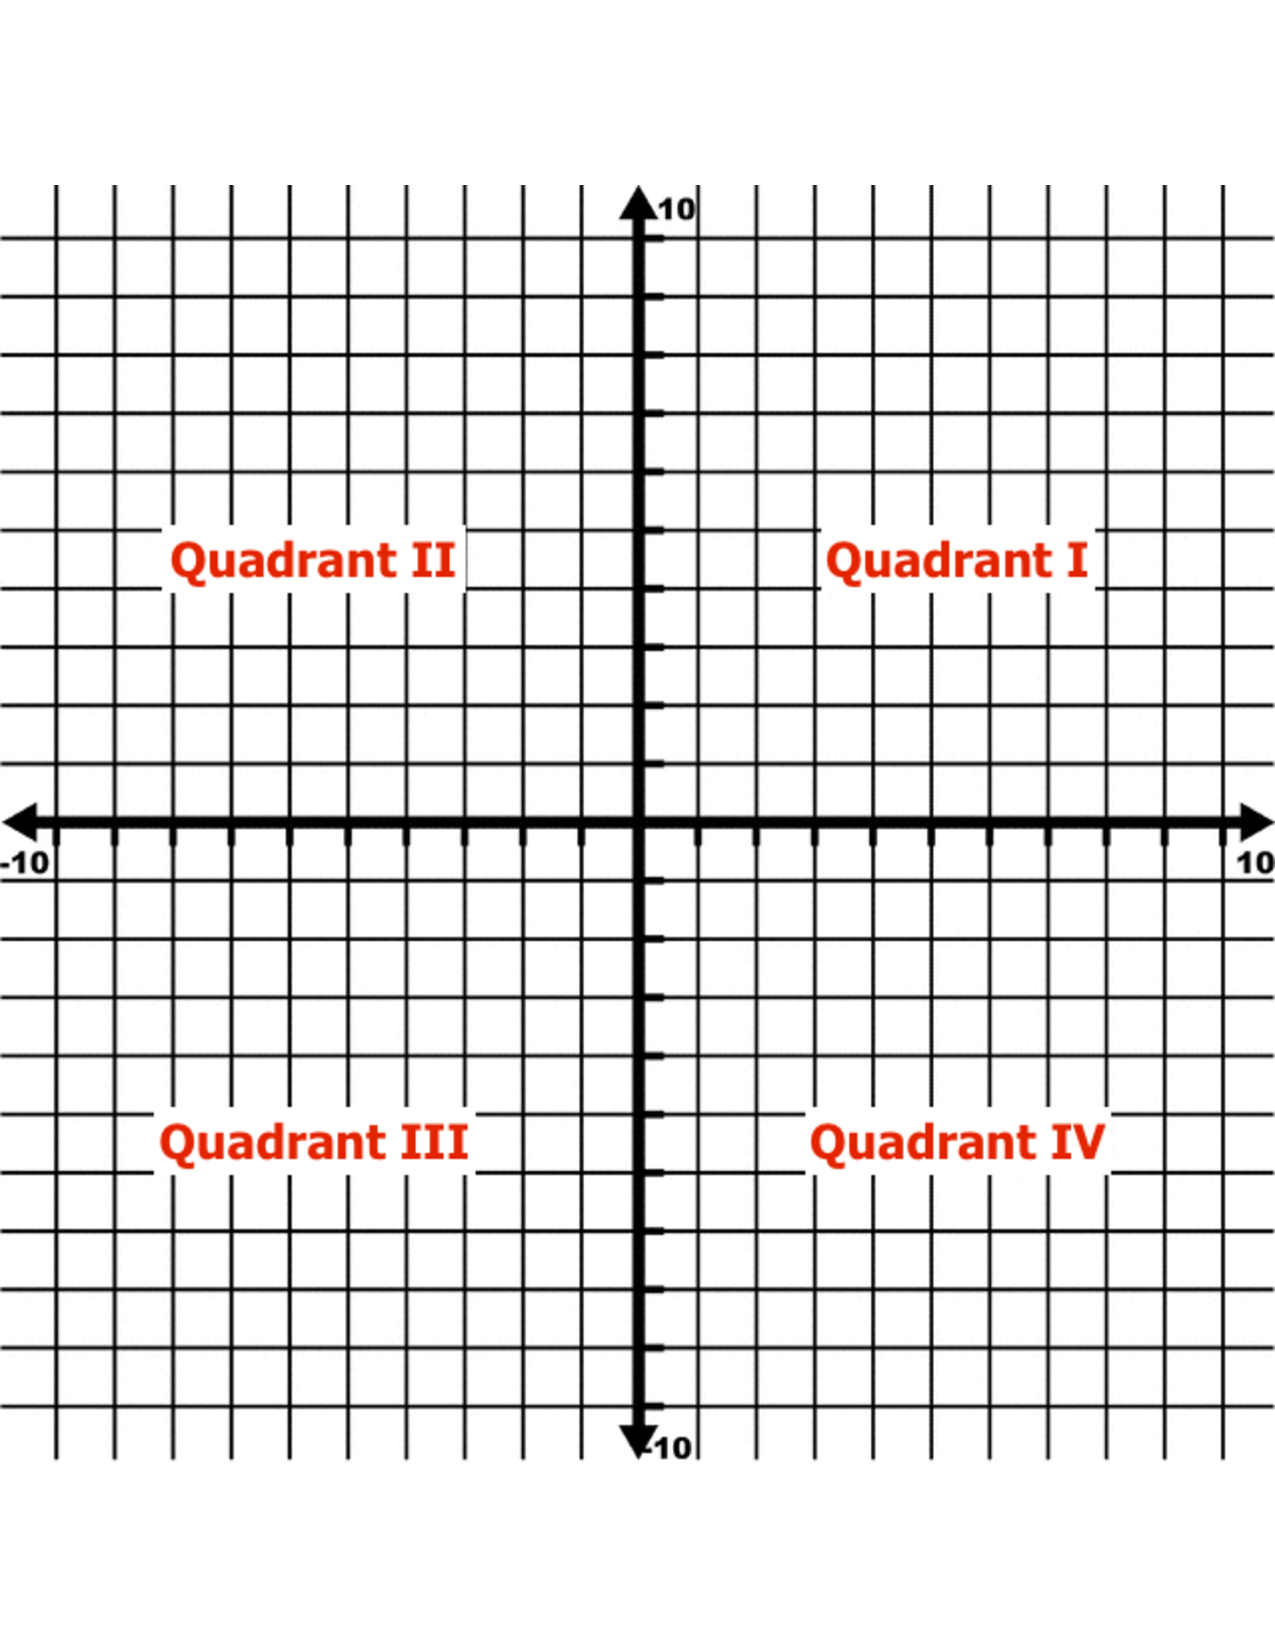
\includegraphics[scale=0.15, trim=-450 100 0 50]{img/coordplan_quadlab.pdf}
        \begin{itemize}
            \item<2-> Points on the coordinate plane are represented as couples of numbers, e.g. $P_1 = (x_1, y_1)$
            \item<3->             
\textbf{Distance Formula:} The distance between two points $P_1 = (x_1, y_1)$ and $P_2 = (x_2, y_2) $ in the x-y plane is given by:
\begin{equation*}
|P_1P_2| = \sqrt[]{(x_2-x_1)^2+(y_2-y_1)^2}
\end{equation*}
        \end{itemize}
    \end{frame}

    \begin{frame}{Exercises}
        \begin{enumerate}
            \item Can you plot the points (1,2) and (3,-2) on the coordinate plane and find the distance between them?
            \item Demonstrate that the Pythagorean Theorem and the distance formula are equivalent. Remember, the PT says:  in a right triangle, where a and b are the lengths of sides next to the right angle, and c is the length of the hypotenuse, the lengths have the relationship
        \end{enumerate}
        $$a^2 + b^2 = c^2$$
   \end{frame}
    \subsection{Lines}

    \begin{frame}{Lines}
       \begin{itemize}
            \item<2-> \textbf{Slope}: The slope of a line passing through the points $P_1 = (x_1, y_1)$ and $P_2 = (x_2, y_2) $ is 
                \begin{equation*}
                    m=\displaystyle \frac{\Delta y}{\Delta x}  = \displaystyle \frac{y_2 - y_1}{ x_2 - x_2} = \displaystyle \frac{rise}{run}
                \end{equation*}
            \item<3->\textbf{Equation of a Line:}
                \begin{enumerate}
                    \item<4-> \textbf{Point-Slope Form:} Given a point, $P_1 = (x_1, y_1)$, and a slope, m, you can plot the line:
                        \begin{equation*}
                            y-y_1 = m(x - x_1)
                        \end{equation*}
                    \item<5-> \textbf{Slope-Intercept Form:} Given a slope, m, and the y-intercept, (0,b), you can plot the line:
                        \begin{equation*}
                        y = mx + b
                        \end{equation*}

                     \onslide<6->{Two lines are parallel if and only if they have the same slope. \\}
                     \onslide<7->{Two lines are perpendicular if and only if their slopes, $m_1$ and $m_2$, are negative reciprocals, i.e. $m_1m_2 = -1$, $m_1 =\frac{-1}{m_2}$}
                \end{enumerate}
       \end{itemize}
    \end{frame}

    \begin{frame}{Linear Regression:}
        \begin{itemize}
              \item<2-> Linear relationships form the basis of much quantitative education research. For a dependent variable, $Y$, with a single independent variable, $X$, we can write:
    $$ Y = \beta_0 + \beta_1 X$$
              \item<3-> We interpret this as ``A one unit change in $X$ is associated with a $\beta_1$ unit change in $Y$.''
              \item<4-> This works for multiple independent variables, too!
              \item<5-> To learn more about this, take EDUC400B, EDUC430A, EDUC430B, or equivalent courses in other departments.
        \end{itemize}
    \end{frame}

    \begin{frame}{Exercises}
        \begin{enumerate}
            \item Plot the line through the points $(1,2)$ and $(4,3)$. 
            \begin{enumerate}
                \item What is the slope? 
                \item What is the intercept?
            \end{enumerate}
            \item A researcher runs a regression of SAT Math score on age and finds the relationship: $$SAT_{Math,i} = 30 \times AGE_i$$.
            \begin{enumerate}
                \item What does this relationship mean, in words?
                \item What problems do you see with the results of this regression?
            \end{enumerate}
        \end{enumerate}
    \end{frame}

    \subsection{Polynomials}

    \begin{frame}{Polynomials}
        \textbf{Definition:} A polynomial is a mathematical expression of one or more terms, where each term is a constant multiplied by one or more variables each raised to a nonnegative integer power. For example: $ax^2 + bx + c$. \\
        
        \onslide<2->{\textbf{Terminology:}}
            \begin{itemize}
                \item<3-> \textbf{Degree:} The degree of a polynomial is the highest degree of its terms. The degree of a term is the sum of the exponents on the variables. For example, the degree of $ax^2 + bx + c$ is $2$.
                \item<4-> \textbf{Root:} The roots of a polynomial function $f(x)$ are the values of the variable $x$ where $f(x)=0$.  
            \end{itemize}
        \onslide<5->{To find the roots (or zeros) of the quadratic polynomial equation $y=ax^2 + bx + c$, use the \textbf{quadratic equation} $$x = \frac{-b \pm \sqrt[]{b^2-4ac}}{2a}$$}
    \end{frame}

    \begin{frame}{Exercises}
        \begin{enumerate}
            \item Find the roots of: $y=x^2 - 6x + 8$
        \end{enumerate}
    \end{frame}

\section{Limits}
    \begin{frame}{Limits}
        \begin{itemize}

            \item<2->\textbf{Intuitive definition:}
                \onslide<3->{The \textbf{limit} of $f(x)$, as $x$ approaches $a$, equals $L$ if, as we take values closer and closer to $a$ (just a bit bigger and a bit smaller, but not equal to $a$), we can make the values of $f(x)$ arbitrarily close to $L$.}
            \item<4->\textbf{Precise definition:}
                \onslide<5->{Let $f$ be a function defined on some open interval that contains the number $a$ (the function need not be defined at $a$ itself). Then we say the limit of $f(x)$ as $x$ approaches $a$ is $L$ and write
\[\lim_{x\to a} f(x) = L \] if for every number $\varepsilon > 0$ there is a corresponding number $\delta > 0$ such that $|f(x) - L| < \varepsilon$ whenever $0 < |x-a| < \delta$.}
        \end{itemize}
    \end{frame}

    \begin{frame}{Left and Right-handed Limits}
        \begin{itemize}
            \item<2->\textbf{Left-hand limit of $f(x)$}
                Writing $\lim_{x \to a^-}f(x)=L$ means that the left-hand limit of $f(x)$ as $x$ approaches $a$ is equal to $L$ if we can make values of $f(x)$ as close to $L$ as we like by taking $x$ to be sufficiently close to $a$ and $x$ less than $a$. 

            \item<3->\textbf{Right-hand limit of $f(x)$}
Writing $\lim_{x \to a^+}f(x)=L$ means that the right-hand limit of $f(x)$ as $x$ approaches $a$ is equal to $L$ if we can make values of $f(x)$ as close to $L$ as we like by taking $x$ to be sufficiently close to $a$ and $x$ greater than $a$. 

        \item<4->\textbf{Recognize:}
            \[\lim_{x\to a} f(x) = L \quad \textbf{if and only if} \lim_{x \to a^-}f(x) = L \; \textbf{and} \lim_{x \to a^+}f(x)=L \]
        \end{itemize}
    \end{frame}
    \subsection{Properties}
    \begin{frame}{Limit Laws}
Suppose that $c$ is a constant and that the limits $\lim_{x\to a} f(x) \quad \text{and} \quad \lim_{x\to a} g(x)$ exist. Then, the following rules hold:
\begin{enumerate}
\item<2-> $\lim_{x\to a}[f(x) + g(x)] = \lim_{x\to a}f(x) + \lim_{x\to a}g(x) $
\item<3-> $\lim_{x\to a}[f(x) - g(x)] = \lim_{x\to a}f(x) - \lim_{x\to a}g(x) $
\item<4-> $\lim_{x\to a}[cf(x)] =  c\lim_{x\to a}f(x) $
\item<5-> $\lim_{x\to a}[f(x)g(x)] = \lim_{x\to a}f(x) \times \lim_{x\to a}g(x) $
\item<6-> $\displaystyle \lim_{x\to a}\frac{f(x)}{g(x)} = \frac{\displaystyle \lim_{x\to a}f(x)}{\displaystyle \lim_{x\to a}g(x)}$ if $\lim_{x\to a}g(x) \neq 0$
\item<7-> $\lim_{x\to a}[f(x)]^n = [\lim_{x\to a} f(x)]^n$, where $n$ is a positive integer.
\item<8-> $\lim_{x \to a} c = c$
\item<9-> $\lim_{x \to a} x = a$
\item<10-> $\lim_{x \to a} x^n = a^n$, where $n$ is a positive integer. 
\item<11-> $\lim_{x \to a} \sqrt[n]{x} = \sqrt[n]{a}$, where $n$ is a positive integer. Note: If $n$ is even, we assume that $a>0$. 
\item<12-> $\lim_{x \to a} \sqrt[n]{f(x)} = \displaystyle \sqrt[n]{\lim_{x \to a} f(x)}$, where $n$ is a positive integer. If $n$ is even, we assume that $\lim_{x \to a} f(x) >0$. 
\end{enumerate}
\end{frame}

    \begin{frame}{Limit Properties}
        \begin{itemize}
            \item<2->\textbf{Direct Substitution Property:}
            If $f$ is a polynomial or a rational function and $a$ is in the domain of $f$, then 
                \begin{equation*}
                    \lim_{x \to a} f(x) = f(a)
                \end{equation*}

            \item<3->\textbf{Infinite Limits:} $\lim_{x \to a} f(x) = \infty$ means that values of $f(x)$ can be made arbitrarily large by taking $x$ sufficiently close to $a$ but not equal to $a$.

            \item<4->\textbf{Limits at Infinity:} Let $f$ be a function defined on some interval $(a, \infty)$. Then $\lim_{x \to \infty} f(x) =L$ means that values of $f(x)$ can be made as close to $L$ as we like by taking $x$ sufficiently large. 
            \end{itemize}
        \end{frame}

    \begin{frame}{Continuity}
        A function $f$ is continuous at a number $a$ if
                \begin{equation*}
                    \lim_{x \to a} f(x) = f(a)
                \end{equation*}
            \onslide<2->{Special types of continuity:}
            \begin{itemize}
                \item<3->\textbf{Continuous from the right:}
                    A function $f$ is continuous \textit{from the right} at a number $a$ if
                    \begin{equation*}
                        \lim_{x \to a^+} f(x) = f(a)
                    \end{equation*}
                \item<4->\textbf{Continuous from the left:}
                    A function $f$ is continuous \textit{from the left} at a number $a$ if
                    \begin{equation*}
                        \lim_{x \to a^-} f(x) = f(a)
                    \end{equation*}
                \item<5->\textbf{Continuous on an interval:}
                    A function is continuous on an interval if it is continuous at every number in the interval.
            \end{itemize}
    \end{frame}

    \begin{frame}{Exercises}
        \begin{enumerate}
            \item Let $y=x$. Does the limit as $x \to 4$ exist? If it exists, find the limit.
            \item Let 
                \begin{equation*}
                     y=\begin{cases}
                         1, & \text{if $x<1$}\\
                         x^2, & \text{if $x \geq 1$}
                     \end{cases}
                \end{equation*} 
                Does the limit as $x \to 1$ exist? If it exists, find the limit.
            \item Let
                \begin{equation*}
                    y=\begin{cases}
                        x, & \text{if $x\neq2$}\\
                        4, & \text{if $x = 2$}
                    \end{cases}
                \end{equation*} 
                Does the limit as $x \to 2$ exist? If it exists, find the limit.
        \end{enumerate}
    \end{frame}

    \begin{frame}{Done for today!}
        \begin{center}
            Thank you!\\ 
            Homework will be posted on GitHub immediately after class. \\
            See you tomorrow!\\
        \end{center}
    \end{frame}



\end{document} 
